\section{Understanding the Methods}

\subsection{Problem A} 

\paragraph{Problem}
Explain in your report why the first move of the agent for the example search
problem from Figure \ref{fig:figure8} is the east rather than then north given
that then agent does not know initially which cells are blocked.

\begin{figure}[h!]
  \centering
  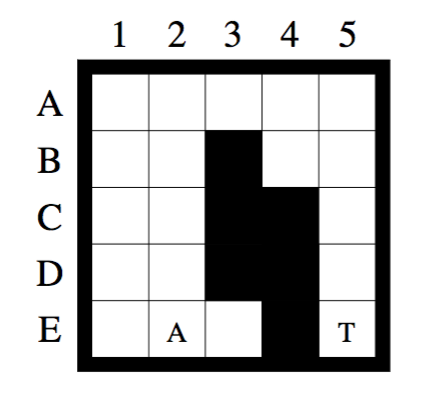
\includegraphics[width=0.4\textwidth]{figure8.png}
  \caption{Second Example Search Problem}
  \label{fig:figure8}
\end{figure}

\paragraph{Solution}
In Figure \ref{fig:figure8}, the start state $A$ is at $(E,2)$ and goal state
$T$ is at $(E,5)$. Let's denote $A_N$ as the north cell $(D,2)$ of $A$, so
$g(A_N)=1$ and $h(A_N)=4$, where $h(A_N)$ is calculated as Manhattan distance
from $A_N$ to $T$. Then, we have
\begin{equation*}
  f(A_N) = g(A_N) + h(A_N) = 5 
\end{equation*}

Equivalently, let's denote $A_E$ as the east cell $(E,3)$ of $A$, so
$g(A_E)=1$, and $h(A_E)=2$. Then
\begin{equation*}
  f(A_E) = g(A_E) + h(A_E) = 3
\end{equation*}

For each iteration in ComputePath, the state with smaller $f-value$ will be
chosen from the $OPEN$ list. In this case, $A_E$ is chosen since
$f(A_E)<f(A_N)$, the agent will first move to the east rather than to the
north.

\subsection{Problem B}

\paragraph{Problem}
This project argues that the agent is guaranteed to reach the target if it is
not separated from it by blocked cells. Give a convincing argument that the
agent in finite gridworlds indeed either reaches the target or discovers that
this is impossible in finite time. Prove that the number of moves of the agent
until it reaches the target or discovers that this is impossible is bounded
from above by the number of unblocked cells squared.

\paragraph{Solution}
For the first question, a finite gridworld can be seen as an undirected graph,
which is divided by the blocked cells into several connected components. The
start cell of agent and the goal must be assigned to any of these connected
components. In one connected component, every cell is reachable from all other
cells in the component. This means an agent can use search algorithms like DFS
or A* to traverse all the cells in the same connected component in finite time.
If start cell and goal cell lie on the same component, the agent can definitely
reach the goal, otherwise, it is impossible for agent to reach the goal after
all the cells are traversed.

For the second question, suppose there are totally $K$ unblocked cells in a
map. Now, let's consider the number of moves in each iteration. For the 1st
iteration, the agent will just move from the start cell to a nearby cell, so
the number of moves is 1. For the 2nd iteration, the agent may either move to
an adjacent new cell or trace back to the start cell and move to the other new
cell next to the start cell, so the largest number of moves is 2. Generally,
for the $i$th iteration, the agent will visit exact one new cell, where a "new
cell" is said to be the cell that has never been visited in previous $i-1$
iterations. Therefore, the largest number of moves is $i$. Since there are
$K$ unblocked cells, there are only $K-1$ iterations. The worst case is that
in each iteration, the agent always traverse the longest path to reach the new
cell. Let's denote $N(k)$ as the total number of moves after $i$th iteration 
and we have

\begin{equation*}
  N(k)=\sum_{i=1}^{i=k-1}=\frac{k(k-1)}{2}=O(k^2)
\end{equation*}

If the start cell and the goal cell are in the same connected component of the
map, $k=K$ so that $N(k)=N(K)=O(K^2)$, otherwise, $k<K$ so that
$N(k)<N(K)=O(K^2)$.  Therefore, in the end, the number of moves of the agent is
bounded from above by the number of unblocked cells squared.
